\documentclass{standalone}
\usepackage{xcolor}
\usepackage{verbatim}
\usepackage{tikz}
\usepackage[T1]{fontenc}
\usepackage{graphics}
\usepackage{hyperref}
\newcommand{\code}[1]{\texttt{#1}}
\newcommand{\R}{R}
\newcommand{\pkg}[1]{#1}
\newcommand{\CRANpkg}[1]{\pkg{#1}}%
\newcommand{\BIOpkg}[1]{\pkg{#1}}
\usepackage{xspace} % Required for \TikZ command

%% load any required packages here
\usepackage{comment}
%\usepackage{todonotes}
\usepackage{multirow}
\usepackage[normalem]{ulem}
\usetikzlibrary{plotmarks}
\usepackage{booktabs}
\usepackage{multirow}
\providecommand{\TikZ}{Ti\textit{k}Z\xspace}
\providecommand{\hyp}{-}
\providecommand{\mean}{\overline}
\begin{document}
\nopagecolor\begin{table}[t!]
\centering
\begin{tabular}{clrrrr}
\toprule
\multirow{2}{*}{Comp.} & \multirow{2}{*}{Data} & \multicolumn{4}{c}{Outputs} \\
\cmidrule(l){3-6}
 &  & R & G & B & RGB\\
\midrule
\multirow{3}{*}{1v2}
 & $t$-test & \uuline{2e-04} & \uuline{0.001} & \uline{0.033} & \uuline{0.002}\\
 & $U$ test & \uuline{8e-05} & \uuline{5e-04} & \uline{0.024} & \uuline{0.001}\\
 & PCS & \raisebox{-.5\height}{\resizebox {1.2cm} {1.2cm} { 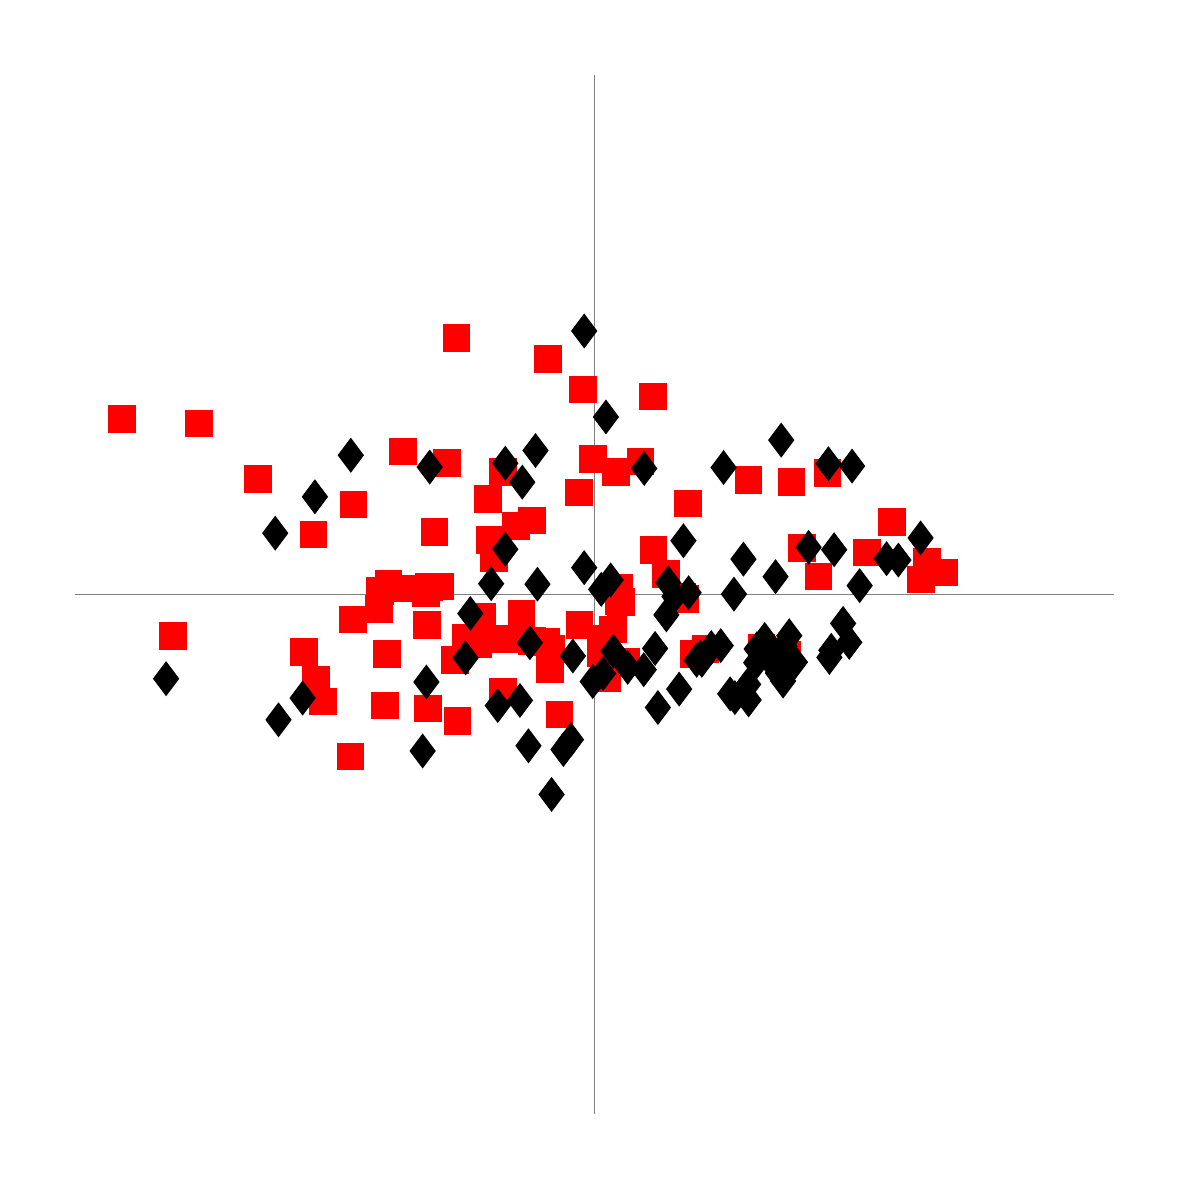
\begin{tikzpicture}[scale=6] \path (-1.2,-1.2) (1.2,1.2);\draw[very thin,color=gray] (0,1.1)--(0,-1.1); \draw[very thin,color=gray] (1.1,0)--(-1.1,0); \path plot[mark=square*,mark options={color=red},mark size=0.8pt] coordinates { (-0.226,0.203) (0.123,0.419) (0.026,-0.177) (0.235,-0.115) (-0.074,-0.254) (-0.238,-0.048) (-0.712,0.244) (0.439,0.098) (0.474,0.038) (-0.327,0.017) (0.066,-0.143) (0.197,0.193) (-0.401,0.013) (-1.000,0.372) (-0.166,0.145) (-0.099,0.498) (-0.102,-0.101) (0.691,0.032) (0.185,-0.005) (-0.444,-0.235) (-0.575,-0.226) (-0.517,-0.343) (-0.457,-0.031) (-0.838,0.362) (-0.222,0.115) (-0.296,-0.138) (-0.025,0.434) (-0.155,-0.041) (0.021,-0.093) (0.407,-0.128) (0.191,-0.010) (-0.189,-0.094) (-0.032,-0.065) (-0.510,0.191) (-0.454,0.007) (-0.511,-0.053) (-0.339,0.133) (-0.133,0.157) (0.056,-0.015) (0.051,0.015) (-0.595,0.127) (-0.350,0.016) (-0.436,0.022) (-0.405,0.303) (-0.353,-0.241) (-0.313,0.279) (-0.589,-0.181) (-0.357,0.002) (-0.615,-0.122) (0.353,-0.113) (0.211,-0.126) (0.704,0.070) (0.013,-0.123) (-0.095,-0.158) (-0.092,-0.115) (0.326,0.243) (-0.290,-0.267) (-0.246,-0.105) (-0.194,-0.205) (-0.892,-0.088) (0.039,-0.074) (0.493,0.257) (0.740,0.047) (0.046,0.260) (0.151,0.044) (-0.133,-0.098) (0.417,0.238) (-0.355,-0.064) (0.125,0.094) (0.576,0.089) (-0.440,-0.126) (-0.004,0.287) (-0.194,0.260) (-0.273,-0.092) (-0.033,0.216) (0.051,-0.013) (0.630,0.153) (-0.213,0.078) (0.097,0.282) (-0.292,0.543)};  \path plot[mark=diamond*,mark size=1pt] coordinates { (-0.205,-0.235) (-0.004,-0.184) (-0.050,-0.307) (0.169,-0.004) (-0.516,0.295) (0.034,0.031) (-0.046,-0.130) (0.128,-0.114) (-0.669,-0.265) (0.539,-0.101) (0.188,0.114) (0.507,0.095) (0.024,0.376) (-0.349,0.270) (-0.907,-0.178) (-0.140,-0.320) (-0.364,-0.331) (-0.066,-0.328) (-0.158,-0.224) (0.388,-0.166) (0.326,-0.223) (0.380,-0.143) (0.497,-0.133) (0.373,-0.141) (-0.137,-0.102) (0.216,-0.139) (0.325,-0.190) (0.134,-0.239) (0.018,-0.167) (-0.219,0.023) (0.383,0.038) (0.526,-0.061) (0.247,-0.112) (0.104,-0.159) (-0.273,-0.134) (-0.022,0.558) (-0.676,0.130) (0.040,-0.120) (-0.091,-0.423) (-0.356,-0.185) (-0.263,-0.040) (0.412,-0.087) (0.014,0.011) (0.295,0.001) (0.156,0.025) (0.199,0.004) (0.643,0.073) (0.287,-0.210) (0.273,0.269) (0.399,-0.183) (0.342,-0.144) (0.267,-0.108) (0.343,-0.115) (0.501,-0.118) (0.152,-0.043) (0.227,-0.139) (-0.121,0.022) (0.179,-0.200) (0.424,-0.143) (0.360,-0.095) (-0.592,0.207) (0.070,-0.154) (0.224,-0.133) (0.561,0.019) (0.495,0.277) (-0.022,0.057) (0.315,0.075) (0.618,0.076) (0.297,-0.218) (0.453,0.100) (0.545,0.272) (0.105,0.267) (0.402,-0.109) (0.690,0.120) (0.395,0.327) (-0.125,0.305) (-0.189,0.096) (-0.618,-0.219) (-0.153,0.238) (-0.189,0.278)};  \end{tikzpicture} }} & \raisebox{-.5\height}{\resizebox {1.2cm} {1.2cm} { 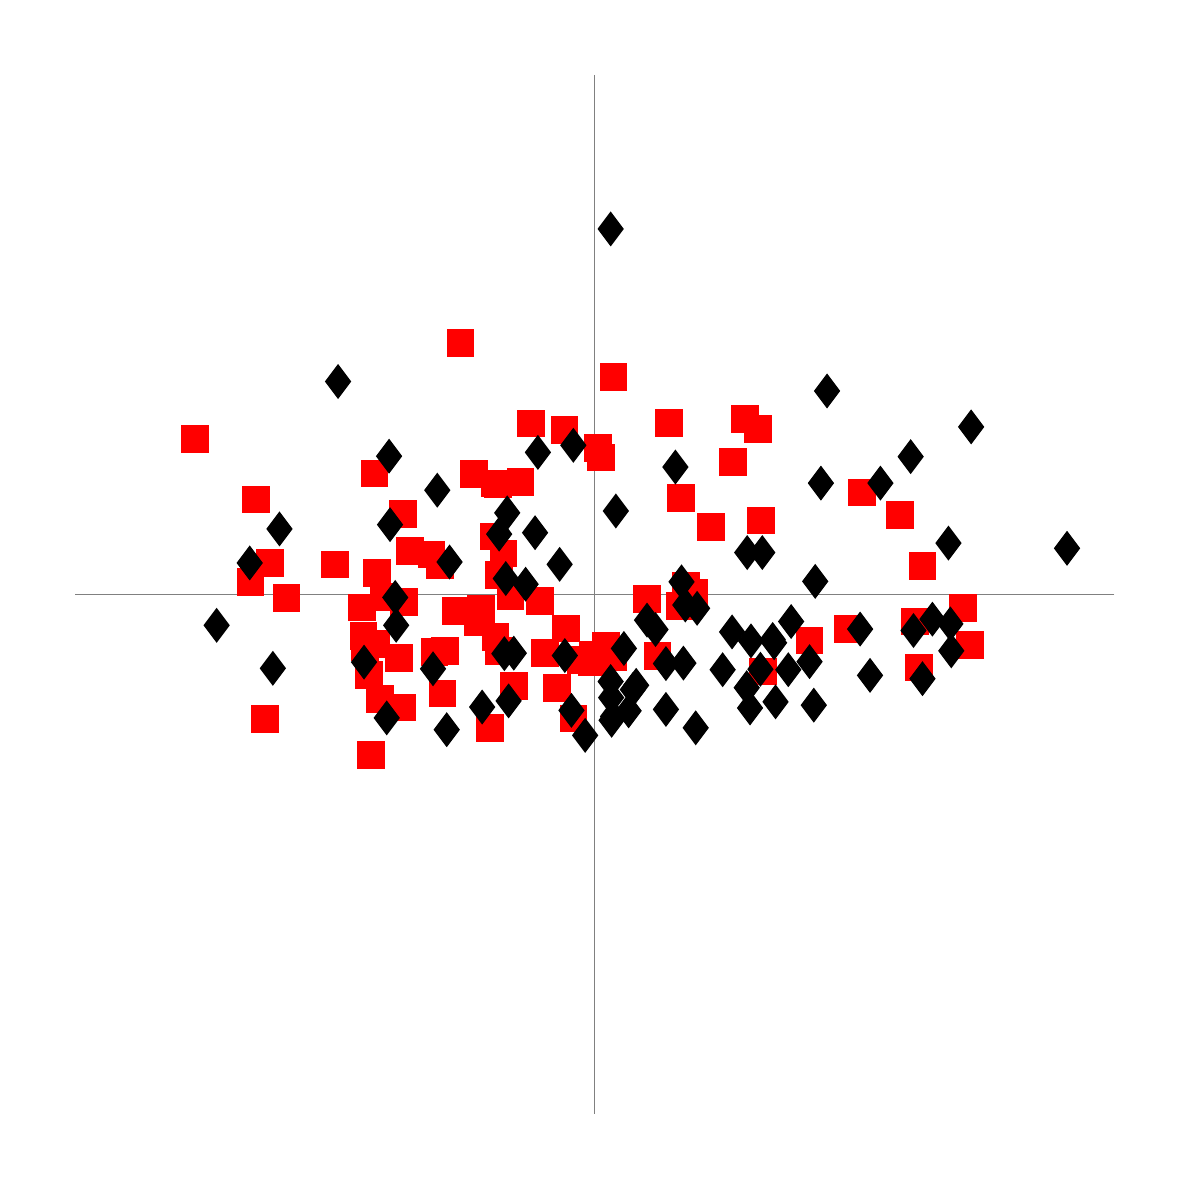
\begin{tikzpicture}[scale=6] \path (-1.2,-1.2) (1.2,1.2);\draw[very thin,color=gray] (0,1.1)--(0,-1.1); \draw[very thin,color=gray] (1.1,0)--(-1.1,0); \path plot[mark=square*,mark options={color=red},mark size=0.8pt] coordinates { (-0.255,0.255) (0.346,0.351) (-0.079,-0.197) (0.455,-0.097) (-0.045,-0.262) (-0.293,-0.035) (0.014,0.290) (0.537,-0.073) (0.687,-0.154) (-0.403,-0.016) (-0.317,-0.120) (0.183,0.205) (-0.406,0.171) (-0.846,0.330) (-0.214,0.123) (0.040,0.461) (-0.493,-0.027) (0.795,-0.107) (0.111,-0.009) (-0.473,-0.339) (-0.486,-0.111) (-0.454,-0.221) (-0.248,-0.058) (-0.717,0.201) (-0.462,-0.104) (-0.203,-0.120) (0.319,0.371) (-0.203,0.041) (0.181,-0.024) (0.356,-0.163) (-0.060,-0.072) (-0.407,-0.239) (0.133,-0.130) (-0.466,0.256) (-0.550,0.064) (-0.728,0.026) (-0.687,0.067) (-0.461,0.046) (-0.241,-0.030) (-0.193,0.087) (-0.345,0.085) (-0.391,0.092) (-0.489,-0.087) (-0.205,0.234) (-0.414,-0.134) (-0.064,0.349) (-0.698,-0.263) (-0.446,-0.005) (-0.477,-0.170) (-0.005,-0.144) (-0.322,-0.209) (0.678,-0.057) (0.024,-0.108) (-0.105,-0.123) (-0.003,-0.127) (0.352,0.157) (-0.221,-0.283) (-0.030,-0.139) (-0.171,-0.194) (-0.652,-0.007) (0.211,0.003) (0.646,0.169) (0.780,-0.028) (0.293,0.280) (0.246,0.143) (0.040,-0.132) (0.566,0.216) (-0.210,-0.090) (-0.327,0.062) (0.158,0.363) (-0.339,-0.122) (-0.157,0.238) (-0.211,0.235) (-0.116,-0.014) (-0.134,0.362) (0.193,0.018) (0.694,0.061) (-0.178,-0.004) (0.007,0.311) (-0.284,0.532)};  \path plot[mark=diamond*,mark size=1pt] coordinates { (-0.049,-0.245) (0.088,-0.192) (-0.238,-0.238) (0.129,-0.074) (-0.543,0.451) (0.111,-0.054) (-0.342,-0.157) (0.331,-0.098) (-0.488,-0.143) (0.410,-0.159) (0.184,0.027) (0.753,-0.062) (0.171,0.270) (-0.333,0.221) (-0.800,-0.065) (0.036,-0.266) (-0.313,-0.286) (-0.020,-0.298) (-0.420,-0.065) (0.329,-0.240) (0.214,-0.282) (0.351,-0.158) (0.455,-0.142) (0.291,-0.079) (-0.171,-0.124) (0.034,-0.184) (0.583,-0.171) (0.322,-0.197) (0.188,-0.145) (-0.433,0.148) (0.467,0.028) (0.755,-0.119) (0.383,-0.227) (0.380,-0.102) (-0.307,0.069) (0.034,0.774) (-0.730,0.067) (0.035,-0.218) (-0.440,-0.261) (-0.422,-0.006) (-0.202,0.128) (0.715,-0.052) (-0.074,0.064) (0.355,0.089) (0.045,0.177) (0.217,-0.029) (0.605,0.236) (0.039,-0.258) (0.323,0.089) (0.464,-0.234) (-0.063,-0.129) (-0.191,-0.125) (0.377,-0.095) (0.694,-0.178) (0.151,-0.146) (0.081,-0.201) (-0.188,0.034) (0.072,-0.246) (0.271,-0.159) (0.562,-0.073) (-0.667,0.139) (0.062,-0.114) (-0.182,-0.225) (0.675,-0.076) (0.492,0.431) (-0.146,0.022) (0.749,0.109) (0.479,0.236) (0.151,-0.243) (0.192,-0.022) (0.797,0.355) (-0.435,0.293) (0.416,-0.057) (1.000,0.098) (0.669,0.292) (-0.045,0.316) (-0.126,0.131) (-0.681,-0.156) (-0.120,0.301) (-0.185,0.173)};  \end{tikzpicture} }} & \raisebox{-.5\height}{\resizebox {1.2cm} {1.2cm} { 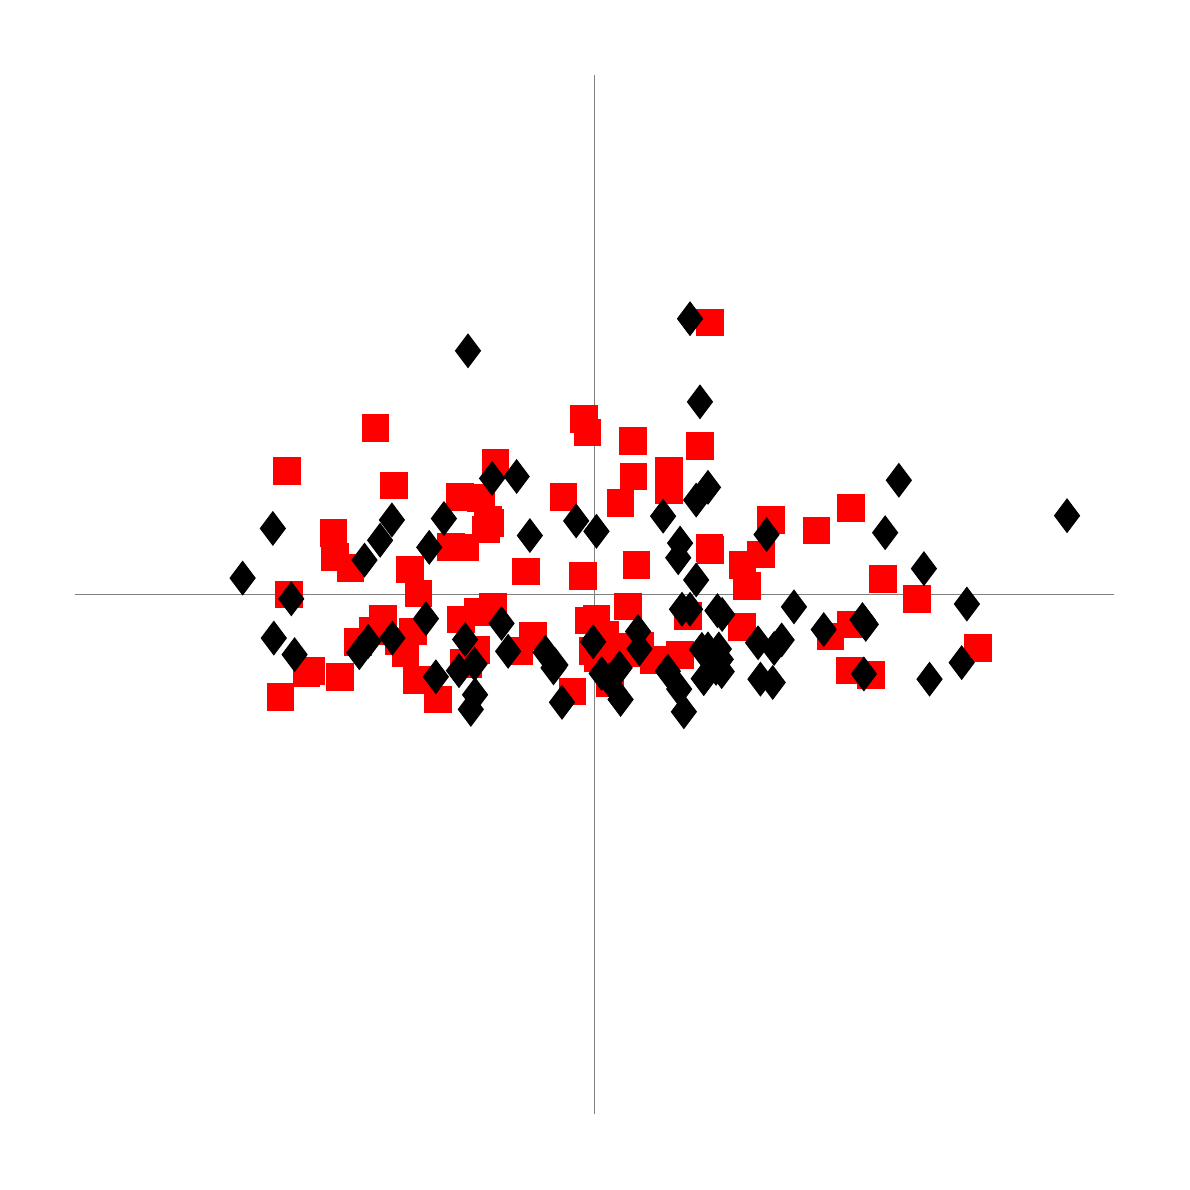
\begin{tikzpicture}[scale=6] \path (-1.2,-1.2) (1.2,1.2);\draw[very thin,color=gray] (0,1.1)--(0,-1.1); \draw[very thin,color=gray] (1.1,0)--(-1.1,0); \path plot[mark=square*,mark options={color=red},mark size=0.8pt] coordinates { (-0.220,0.151) (0.543,0.183) (-0.004,-0.119) (0.543,-0.063) (0.097,-0.108) (-0.304,0.101) (0.245,0.094) (0.540,-0.161) (0.811,-0.113) (-0.248,-0.037) (-0.373,0.002) (0.089,0.062) (-0.241,0.204) (-0.464,0.353) (-0.066,0.206) (0.223,0.314) (-0.517,0.057) (0.585,-0.170) (0.004,-0.051) (-0.331,-0.222) (-0.415,-0.099) (-0.400,-0.124) (0.070,-0.025) (-0.285,0.207) (-0.448,-0.052) (-0.268,-0.148) (0.470,0.136) (-0.145,0.049) (0.198,-0.045) (0.126,-0.138) (-0.385,-0.078) (-0.665,-0.217) (0.033,-0.188) (-0.210,0.279) (-0.425,0.231) (-0.651,0.262) (-0.553,0.131) (-0.391,0.053) (-0.469,-0.077) (-0.225,0.159) (-0.215,-0.025) (-0.550,0.080) (-0.599,-0.162) (0.158,0.263) (-0.283,-0.053) (0.055,0.194) (-0.501,-0.101) (-0.230,0.138) (-0.376,-0.181) (-0.251,-0.117) (-0.539,-0.174) (0.181,-0.128) (0.023,-0.085) (-0.130,-0.088) (0.065,-0.111) (0.323,0.018) (-0.047,-0.205) (0.072,-0.125) (-0.159,-0.120) (-0.274,0.100) (0.352,0.085) (0.682,-0.009) (0.499,-0.089) (0.374,0.158) (0.243,0.099) (0.006,-0.134) (0.611,0.033) (-0.276,-0.145) (-0.647,-0.000) (0.082,0.250) (-0.610,-0.166) (0.081,0.325) (0.157,0.221) (-0.024,0.039) (-0.023,0.371) (-0.012,-0.055) (0.312,-0.068) (0.313,0.063) (-0.015,0.343) (0.244,0.576)};  \path plot[mark=diamond*,mark size=1pt] coordinates { (0.231,-0.178) (0.015,-0.167) (-0.287,-0.161) (0.202,-0.031) (-0.268,0.516) (0.263,-0.115) (-0.679,-0.092) (0.346,-0.102) (-0.274,-0.095) (0.240,-0.115) (0.185,-0.031) (0.777,-0.144) (0.364,0.127) (-0.350,0.100) (-0.642,-0.009) (0.269,-0.163) (-0.197,-0.061) (0.055,-0.222) (-0.487,0.073) (0.267,-0.137) (-0.069,-0.228) (0.258,-0.140) (0.227,-0.116) (0.177,0.078) (-0.104,-0.122) (-0.254,-0.147) (0.351,-0.179) (0.031,-0.181) (0.053,-0.155) (-0.429,0.158) (0.260,-0.034) (0.570,-0.168) (0.189,-0.248) (0.574,-0.063) (-0.165,0.250) (0.202,0.584) (-0.745,0.035) (0.179,-0.200) (-0.498,-0.123) (-0.454,0.115) (-0.319,0.161) (0.380,-0.114) (0.004,0.134) (0.215,0.031) (-0.039,0.156) (-0.003,-0.100) (0.615,0.131) (-0.253,-0.212) (0.422,-0.026) (0.377,-0.186) (-0.479,-0.099) (-0.635,-0.127) (0.485,-0.074) (0.709,-0.179) (0.155,-0.162) (0.095,-0.115) (0.181,0.109) (-0.262,-0.243) (-0.087,-0.155) (0.396,-0.096) (-0.681,0.140) (0.092,-0.078) (-0.336,-0.174) (0.257,-0.156) (0.644,0.242) (-0.357,-0.051) (0.567,-0.053) (0.215,0.200) (-0.083,-0.149) (-0.183,-0.120) (1.000,0.167) (-0.217,0.246) (0.270,-0.042) (0.788,-0.020) (0.697,0.055) (-0.137,0.125) (0.240,0.227) (-0.428,-0.092) (0.223,0.408) (0.145,0.166)};  \end{tikzpicture} }} & \raisebox{-.5\height}{\resizebox {1.2cm} {1.2cm} { 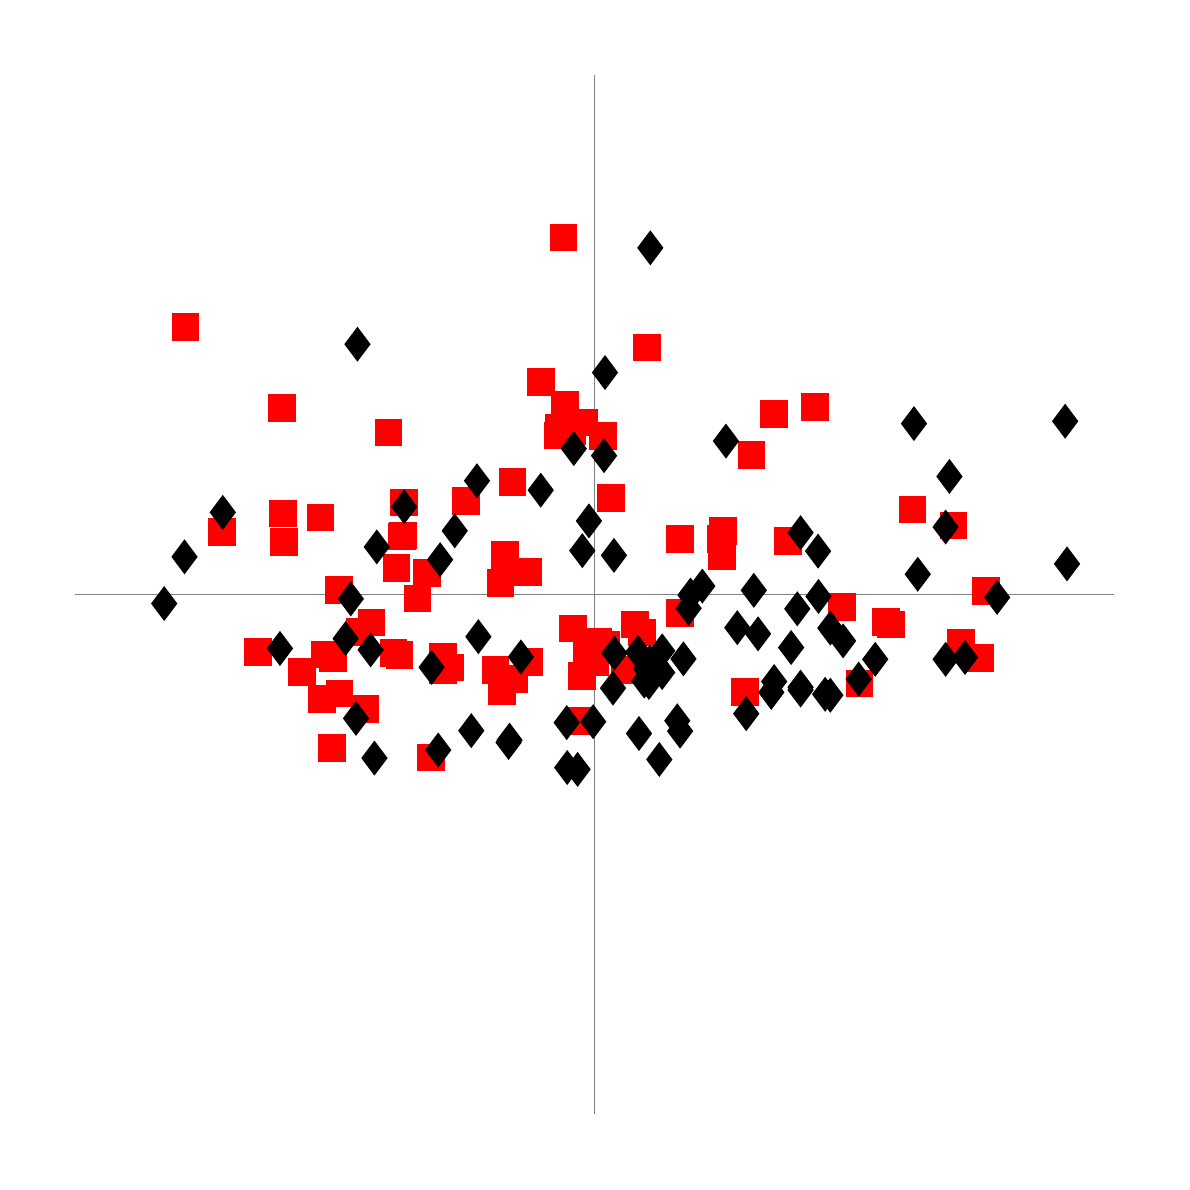
\begin{tikzpicture}[scale=6] \path (-1.2,-1.2) (1.2,1.2);\draw[very thin,color=gray] (0,1.1)--(0,-1.1); \draw[very thin,color=gray] (1.1,0)--(-1.1,0); \path plot[mark=square*,mark options={color=red},mark size=0.8pt] coordinates { (-0.272,0.198) (0.467,0.397) (-0.027,-0.173) (0.524,-0.026) (0.001,-0.142) (-0.355,0.046) (-0.063,0.401) (0.627,-0.063) (0.828,0.007) (-0.375,-0.008) (-0.307,-0.154) (0.181,0.117) (-0.403,0.195) (-0.866,0.566) (-0.174,0.238) (0.111,0.523) (-0.497,-0.079) (0.816,-0.134) (0.101,-0.080) (-0.485,-0.242) (-0.572,-0.127) (-0.540,-0.209) (-0.189,0.084) (-0.661,0.395) (-0.472,-0.059) (-0.305,-0.154) (0.380,0.382) (-0.199,0.024) (0.181,-0.039) (0.318,-0.206) (-0.170,-0.179) (-0.556,-0.325) (0.065,-0.160) (-0.436,0.343) (-0.580,0.163) (-0.789,0.132) (-0.657,0.111) (-0.419,0.056) (-0.321,-0.161) (-0.180,0.048) (-0.408,0.123) (-0.541,0.010) (-0.620,-0.164) (-0.113,0.450) (-0.413,-0.128) (-0.077,0.337) (-0.713,-0.121) (-0.405,0.125) (-0.554,-0.135) (-0.034,-0.267) (-0.346,-0.345) (0.561,-0.188) (0.024,-0.106) (-0.139,-0.142) (0.008,-0.101) (0.409,0.114) (-0.196,-0.204) (-0.046,-0.072) (-0.210,-0.160) (-0.660,0.172) (0.270,0.082) (0.760,0.146) (0.776,-0.103) (0.332,0.296) (0.267,0.117) (-0.017,-0.113) (0.673,0.180) (-0.321,-0.131) (-0.426,-0.124) (0.272,0.134) (-0.577,-0.221) (-0.022,0.364) (-0.048,0.346) (-0.140,0.048) (-0.076,0.354) (0.086,-0.063) (0.617,-0.058) (0.035,0.204) (0.018,0.336) (-0.066,0.756)};  \path plot[mark=diamond*,mark size=1pt] coordinates { (0.042,-0.124) (0.039,-0.198) (-0.261,-0.288) (0.203,-0.001) (-0.502,0.530) (0.199,-0.029) (-0.505,-0.262) (0.346,-0.083) (-0.527,-0.093) (0.436,-0.196) (0.228,0.018) (0.852,-0.006) (0.278,0.325) (-0.403,0.186) (-0.911,-0.019) (0.109,-0.157) (-0.345,-0.154) (-0.003,-0.269) (-0.474,-0.117) (0.374,-0.207) (0.137,-0.349) (0.380,-0.184) (0.436,-0.202) (0.302,-0.070) (-0.156,-0.132) (-0.059,-0.271) (0.499,-0.213) (0.175,-0.267) (0.105,-0.183) (-0.461,0.101) (0.429,-0.030) (0.743,-0.137) (0.321,-0.252) (0.474,-0.004) (-0.296,0.135) (0.118,0.734) (-0.868,0.080) (0.117,-0.143) (-0.466,-0.346) (-0.516,-0.009) (-0.327,0.074) (0.594,-0.137) (-0.026,0.093) (0.337,0.009) (0.041,0.083) (0.143,-0.119) (0.743,0.143) (-0.036,-0.370) (0.436,0.131) (0.488,-0.211) (-0.180,-0.308) (-0.331,-0.329) (0.499,-0.071) (0.784,-0.133) (0.188,-0.136) (0.143,-0.165) (-0.012,0.156) (-0.058,-0.366) (0.181,-0.289) (0.526,-0.098) (-0.787,0.174) (0.092,-0.122) (-0.182,-0.313) (0.559,-0.179) (0.676,0.362) (-0.246,-0.089) (0.684,0.043) (0.473,0.092) (0.094,-0.294) (0.115,-0.186) (0.996,0.367) (-0.249,0.241) (0.416,-0.112) (1.000,0.065) (0.751,0.250) (-0.114,0.221) (0.020,0.294) (-0.666,-0.114) (0.022,0.470) (-0.044,0.309)};  \end{tikzpicture} }}\\
\midrule
\multirow{3}{*}{1v3}
 & $t$-test & \uuline{<1e-08} & \uuline{<1e-08} & \uuline{7e-07} & \uuline{<1e-08}\\
 & $U$ test & \uuline{<1e-08} & \uuline{<1e-08} & \uuline{7e-06} & \uuline{<1e-08}\\
 & PCS & \raisebox{-.5\height}{\resizebox {1.2cm} {1.2cm} { 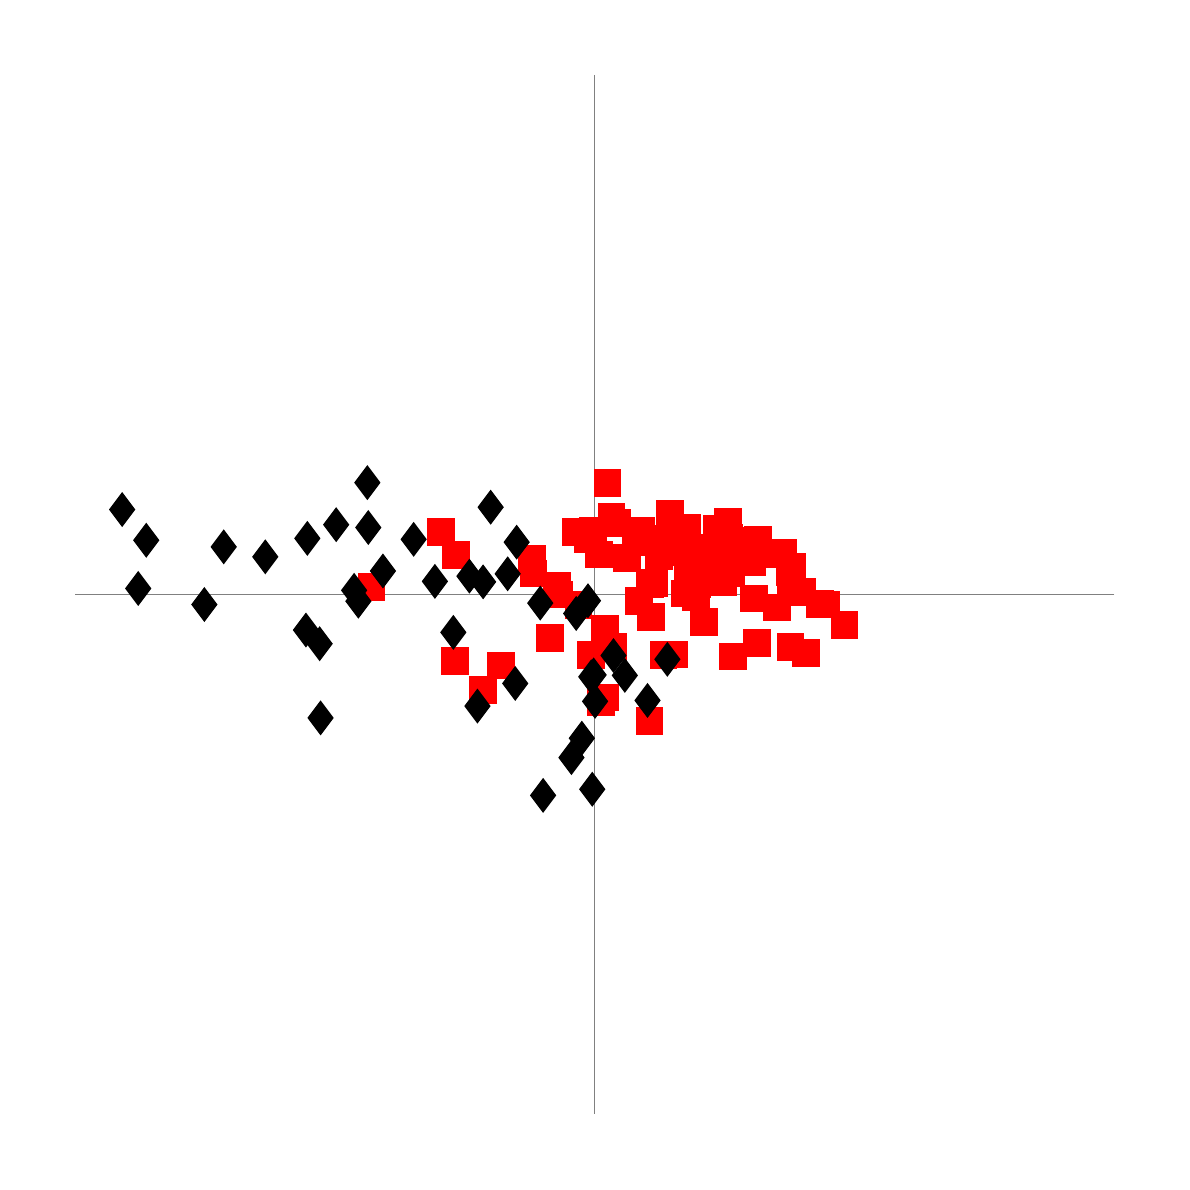
\begin{tikzpicture}[scale=6] \path (-1.2,-1.2) (1.2,1.2);\draw[very thin,color=gray] (0,1.1)--(0,-1.1); \draw[very thin,color=gray] (1.1,0)--(-1.1,0); \path plot[mark=square*,mark options={color=red},mark size=0.8pt] coordinates { (-0.040,0.133) (0.088,0.111) (0.048,0.152) (0.215,-0.005) (-0.198,-0.150) (0.127,0.024) (0.069,0.078) (0.173,0.089) (-0.325,0.132) (0.418,0.058) (0.231,-0.058) (0.416,0.026) (0.146,-0.128) (-0.095,-0.092) (-0.472,0.016) (-0.003,0.134) (-0.133,0.075) (0.036,0.165) (-0.014,0.117) (0.326,0.076) (0.282,0.153) (0.322,0.104) (0.393,0.085) (0.317,0.075) (0.009,0.085) (0.225,0.088) (0.284,0.121) (0.159,0.172) (0.098,0.136) (-0.034,-0.022) (0.338,-0.008) (0.413,0.048) (0.241,0.100) (0.148,0.119) (-0.080,0.018) (0.116,-0.267) (-0.295,-0.140) (0.117,0.023) (0.027,0.236) (-0.129,0.045) (-0.075,0.000) (0.341,0.106) (0.119,-0.048) (0.273,0.027) (0.190,0.002) (0.218,0.023) (0.491,-0.021) (0.259,0.140) (0.293,-0.131) (0.333,0.113) (0.296,0.078) (0.254,0.059) (0.306,0.081) (0.399,0.089) (0.198,0.038) (0.237,0.070) (0.022,-0.073) (0.196,0.141) (0.346,0.115) (0.312,0.088) (-0.236,-0.202) (0.137,0.082) (0.227,0.084) (0.440,0.005) (0.415,-0.111) (0.094,-0.014) (0.289,0.046) (0.477,-0.020) (0.271,0.110) (0.386,-0.027) (0.447,-0.124) (0.168,-0.127) (0.333,0.068) (0.529,-0.065) (0.344,-0.103) (0.039,-0.111) (-0.007,-0.128) (-0.293,0.084) (0.023,-0.218) (0.013,-0.228)};  \path plot[mark=diamond*,mark size=1pt] coordinates { (-0.509,0.009) (-0.220,0.185) (-0.611,-0.075) (-0.826,-0.021) (-0.966,0.013) (-0.785,0.101) (-0.383,0.117) (-0.481,0.237) (-0.547,0.148) (-0.580,-0.261) (-0.248,-0.236) (-0.500,-0.014) (-0.608,0.119) (-0.697,0.080) (-0.236,0.027) (0.001,-0.226) (-0.039,-0.040) (-0.949,0.115) (-0.338,0.028) (-0.184,0.044) (-0.165,0.111) (-0.007,-0.174) (-0.299,-0.080) (-0.168,-0.188) (-0.027,-0.304) (-0.115,-0.018) (0.064,-0.171) (-1.000,0.180) (-0.265,0.039) (-0.479,0.142) (-0.448,0.050) (-0.582,-0.104) (-0.049,-0.345) (0.154,-0.137) (-0.109,-0.425) (-0.005,-0.412) (-0.002,-0.170) (0.040,-0.129) (-0.014,-0.013) (0.112,-0.224)};  \end{tikzpicture} }} & \raisebox{-.5\height}{\resizebox {1.2cm} {1.2cm} { 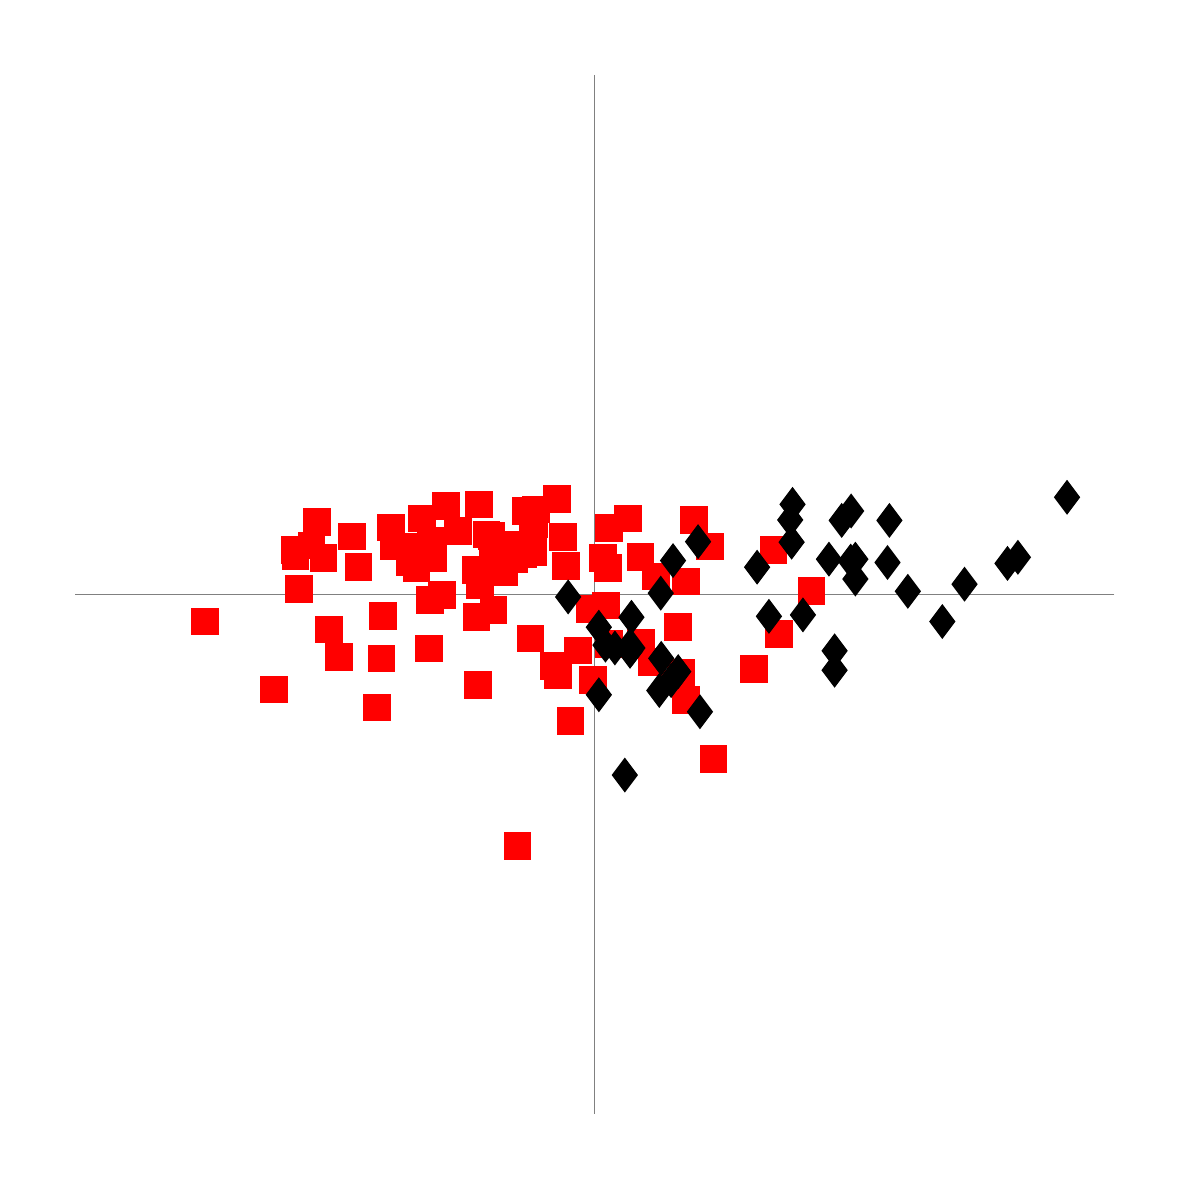
\begin{tikzpicture}[scale=6] \path (-1.2,-1.2) (1.2,1.2);\draw[very thin,color=gray] (0,1.1)--(0,-1.1); \draw[very thin,color=gray] (1.1,0)--(-1.1,0); \path plot[mark=square*,mark options={color=red},mark size=0.8pt] coordinates { (-0.067,0.122) (-0.167,0.105) (0.070,0.161) (-0.214,-0.032) (0.252,-0.348) (-0.191,0.048) (0.130,0.038) (-0.342,0.077) (0.244,0.102) (-0.390,0.102) (-0.250,-0.048) (-0.633,0.081) (-0.247,-0.192) (0.122,-0.143) (0.459,0.007) (-0.128,0.150) (0.097,0.080) (-0.080,0.202) (0.193,0.028) (-0.344,0.087) (-0.244,0.191) (-0.347,0.114) (-0.424,0.102) (-0.323,-0.001) (0.018,0.078) (-0.130,0.089) (-0.514,0.123) (-0.314,0.187) (-0.229,0.127) (0.183,-0.166) (-0.448,-0.045) (-0.635,0.095) (-0.365,0.161) (-0.364,0.099) (0.098,-0.102) (-0.163,-0.532) (0.391,-0.084) (-0.131,0.124) (0.210,0.158) (0.177,-0.068) (0.031,-0.105) (-0.599,0.104) (-0.086,-0.151) (-0.348,-0.012) (-0.136,-0.093) (-0.251,0.052) (-0.541,-0.132) (-0.124,0.180) (-0.351,-0.114) (-0.431,0.142) (-0.061,0.060) (0.028,0.057) (-0.377,0.057) (-0.587,0.153) (-0.216,0.068) (-0.170,0.074) (0.024,-0.023) (-0.145,0.177) (-0.289,0.134) (-0.500,0.058) (0.337,-0.157) (-0.152,0.086) (0.030,0.141) (-0.574,0.078) (-0.461,-0.239) (-0.010,-0.031) (-0.626,0.012) (-0.451,-0.135) (-0.218,0.124) (-0.243,0.021) (-0.678,-0.201) (0.193,-0.223) (-0.391,0.069) (-0.825,-0.057) (-0.562,-0.074) (-0.077,-0.171) (-0.035,-0.118) (0.379,0.095) (-0.051,-0.268) (-0.003,-0.181)};  \path plot[mark=diamond*,mark size=1pt] coordinates { (0.552,0.075) (0.166,0.072) (0.508,-0.160) (0.896,0.079) (0.736,-0.057) (0.663,0.007) (0.419,0.191) (0.414,0.158) (0.543,0.177) (0.508,-0.119) (0.223,-0.248) (0.369,-0.046) (0.552,0.033) (0.624,0.157) (0.344,0.058) (0.080,-0.113) (0.043,-0.113) (0.874,0.066) (0.441,-0.043) (0.542,0.071) (0.417,0.111) (0.009,-0.069) (0.177,-0.163) (0.162,-0.182) (0.141,-0.135) (0.219,0.112) (0.023,-0.107) (1.000,0.206) (0.620,0.068) (0.523,0.157) (0.496,0.075) (0.783,0.022) (0.137,-0.203) (0.140,0.003) (0.064,-0.382) (0.009,-0.212) (0.074,-0.109) (0.078,-0.048) (-0.056,-0.005) (0.075,-0.120)};  \end{tikzpicture} }} & \raisebox{-.5\height}{\resizebox {1.2cm} {1.2cm} { 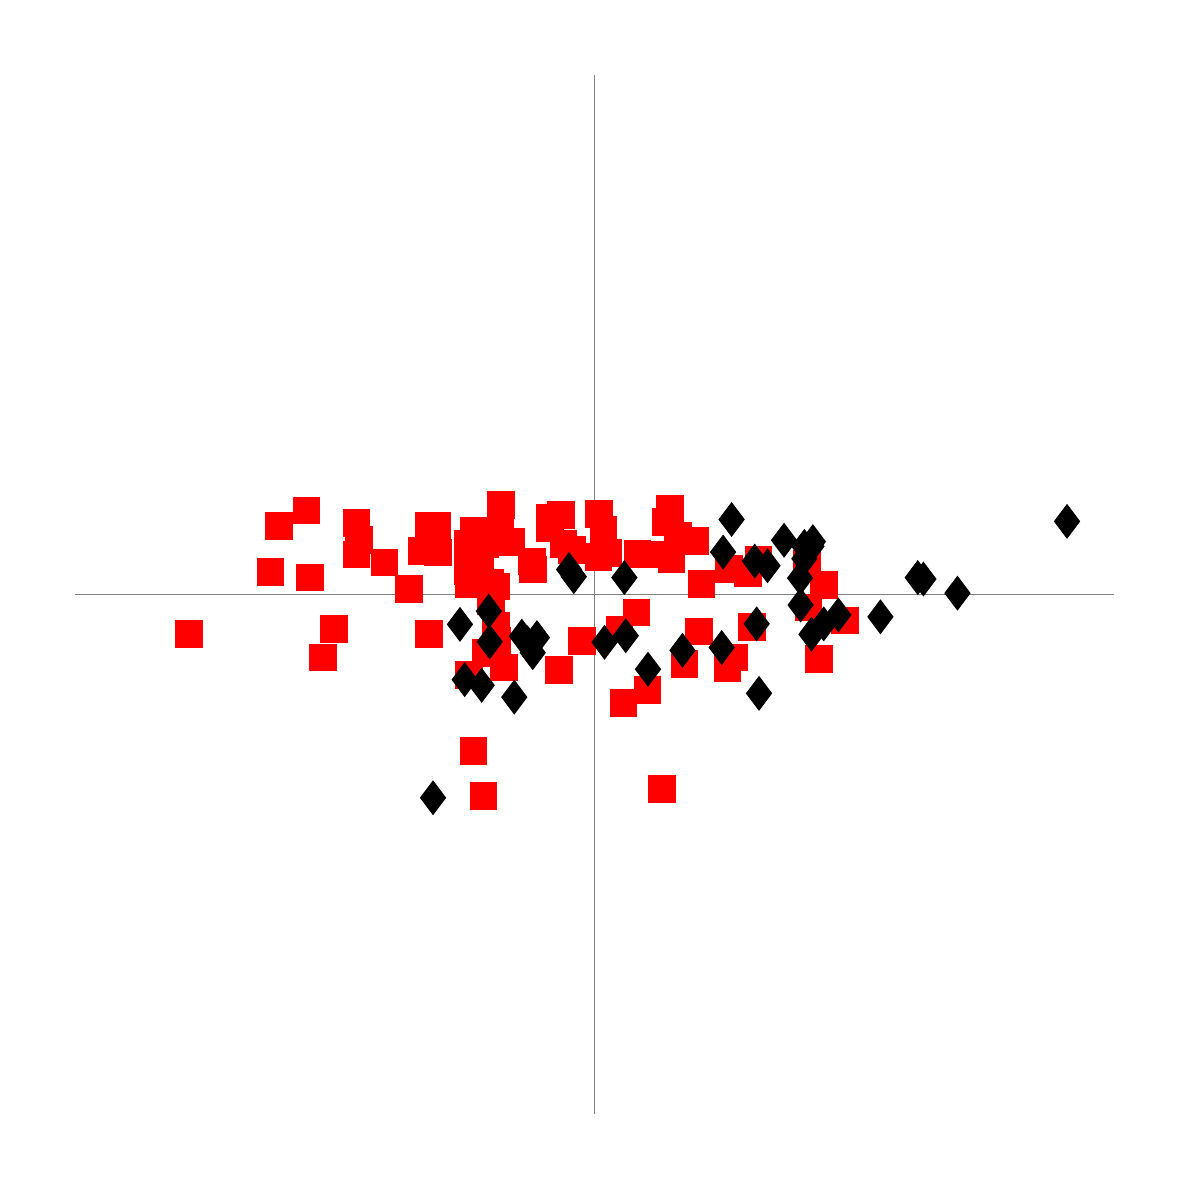
\begin{tikzpicture}[scale=6] \path (-1.2,-1.2) (1.2,1.2);\draw[very thin,color=gray] (0,1.1)--(0,-1.1); \draw[very thin,color=gray] (1.1,0)--(-1.1,0); \path plot[mark=square*,mark options={color=red},mark size=0.8pt] coordinates { (-0.236,0.115) (-0.066,0.107) (0.177,0.124) (-0.219,-0.013) (0.143,-0.411) (-0.269,0.091) (0.485,0.021) (-0.331,0.089) (0.163,0.074) (-0.243,0.083) (-0.208,0.017) (-0.668,0.145) (-0.351,-0.083) (0.221,-0.078) (0.453,-0.027) (-0.269,0.108) (0.089,-0.038) (-0.094,0.162) (0.333,-0.069) (-0.269,0.049) (0.010,0.171) (-0.254,0.122) (-0.232,0.107) (-0.206,-0.097) (0.028,0.088) (0.149,0.085) (-0.333,0.146) (-0.071,0.168) (-0.094,0.140) (0.281,-0.156) (-0.266,0.023) (-0.504,0.152) (-0.198,0.189) (-0.504,0.085) (0.061,-0.229) (-0.235,-0.426) (0.530,-0.055) (-0.199,0.141) (0.347,0.074) (0.295,-0.133) (0.190,-0.147) (-0.350,0.146) (-0.075,-0.159) (-0.221,0.024) (-0.026,-0.098) (-0.048,0.095) (-0.551,-0.073) (0.150,0.154) (-0.393,0.012) (-0.345,0.146) (0.324,0.046) (0.449,0.065) (-0.445,0.068) (-0.610,0.178) (-0.177,0.112) (-0.131,0.053) (-0.209,-0.066) (0.159,0.182) (0.019,0.137) (-0.365,0.092) (0.475,-0.136) (-0.133,0.070) (0.213,0.113) (-0.255,0.134) (-0.575,-0.133) (0.226,0.023) (-0.499,0.115) (-0.230,-0.123) (0.008,0.079) (0.091,0.086) (-0.858,-0.083) (0.112,-0.202) (-0.266,0.068) (-0.686,0.048) (-0.603,0.036) (0.053,-0.074) (-0.266,-0.170) (0.284,0.054) (-0.256,-0.331) (-0.192,-0.154)};  \path plot[mark=diamond*,mark size=1pt] coordinates { (0.459,0.102) (0.063,0.036) (0.348,-0.209) (0.768,0.003) (0.459,-0.084) (0.516,-0.043) (0.290,0.159) (0.272,0.090) (0.401,0.115) (0.343,-0.062) (0.269,-0.112) (0.066,-0.087) (0.436,-0.022) (0.462,0.112) (0.339,0.071) (-0.142,-0.102) (0.021,-0.101) (0.696,0.033) (0.485,-0.062) (0.435,0.035) (0.444,0.102) (-0.285,-0.063) (0.113,-0.158) (0.186,-0.118) (-0.122,-0.091) (-0.054,0.053) (-0.170,-0.217) (1.000,0.155) (0.684,0.036) (0.444,0.076) (0.366,0.061) (0.605,-0.047) (-0.239,-0.192) (-0.154,-0.088) (-0.342,-0.430) (-0.224,-0.035) (-0.222,-0.100) (-0.131,-0.123) (-0.044,0.038) (-0.275,-0.180)};  \end{tikzpicture} }} & \raisebox{-.5\height}{\resizebox {1.2cm} {1.2cm} { 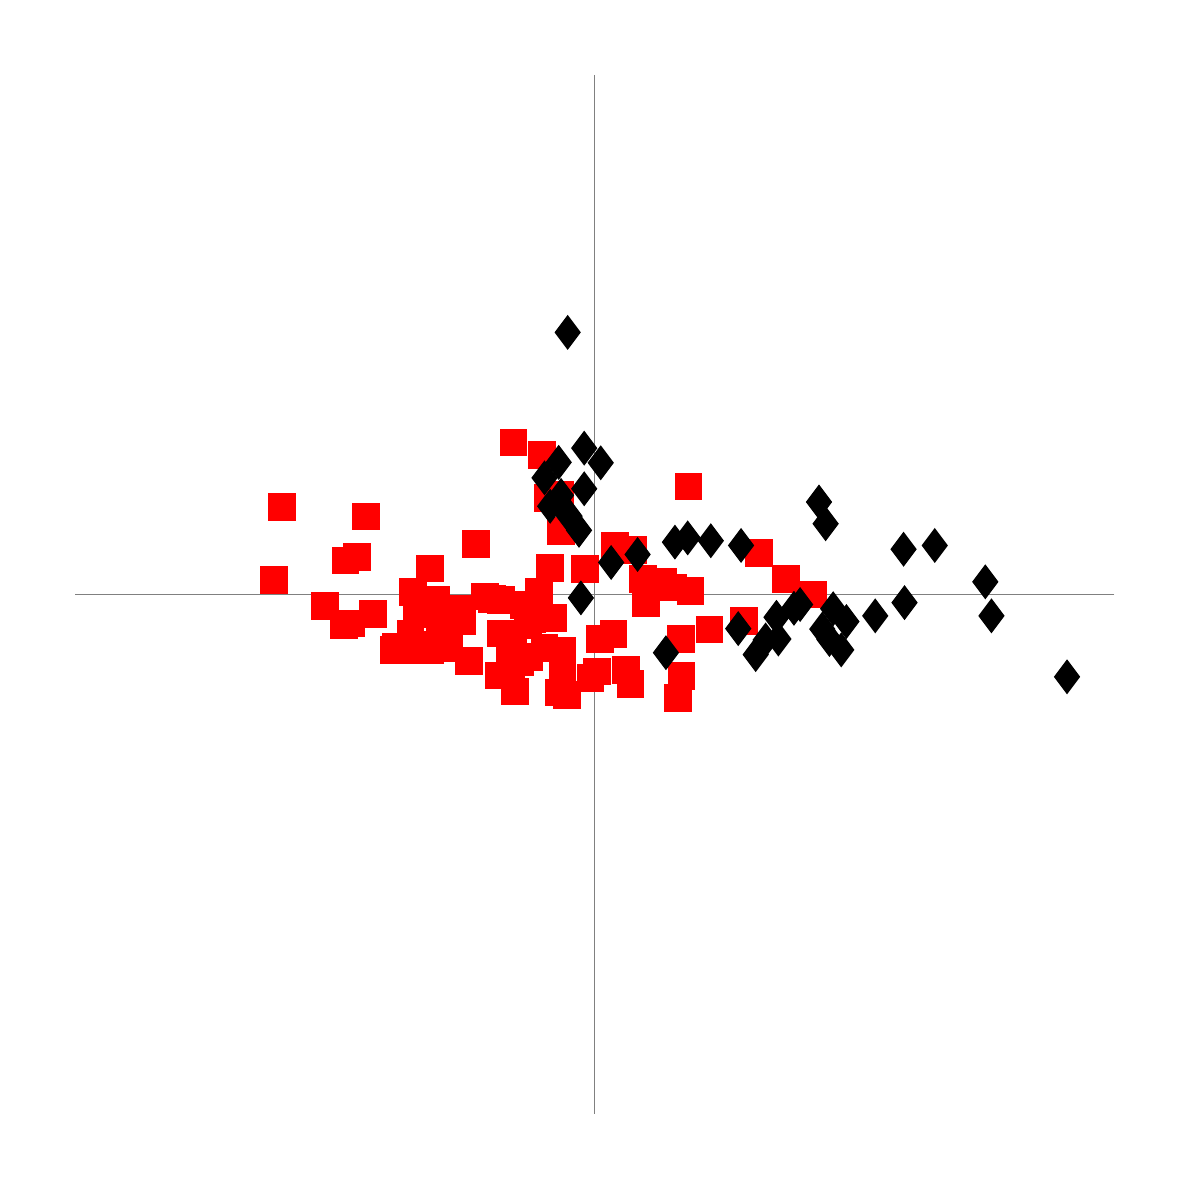
\begin{tikzpicture}[scale=6] \path (-1.2,-1.2) (1.2,1.2);\draw[very thin,color=gray] (0,1.1)--(0,-1.1); \draw[very thin,color=gray] (1.1,0)--(-1.1,0); \path plot[mark=square*,mark options={color=red},mark size=0.8pt] coordinates { (-0.087,-0.049) (-0.106,-0.113) (0.067,-0.159) (-0.217,-0.009) (0.199,0.229) (-0.198,-0.012) (0.184,-0.172) (-0.281,-0.056) (0.243,-0.074) (-0.349,-0.107) (-0.232,-0.004) (-0.571,-0.024) (-0.251,0.107) (0.145,0.026) (0.462,0.000) (-0.132,-0.052) (0.109,-0.018) (-0.068,-0.119) (0.183,-0.094) (-0.312,-0.073) (-0.169,-0.205) (-0.307,-0.113) (-0.348,-0.117) (-0.280,-0.031) (0.011,-0.094) (-0.068,-0.161) (-0.373,-0.109) (-0.176,-0.166) (-0.139,-0.132) (0.167,0.015) (-0.350,-0.032) (-0.515,-0.061) (-0.266,-0.140) (-0.336,-0.012) (0.082,0.094) (-0.172,0.322) (0.405,0.033) (-0.149,-0.022) (0.177,-0.219) (0.203,0.007) (0.102,0.033) (-0.425,-0.117) (-0.094,0.056) (-0.280,-0.040) (-0.117,0.005) (-0.172,-0.095) (-0.527,0.072) (-0.076,-0.207) (-0.348,0.055) (-0.368,-0.117) (-0.009,-0.176) (0.076,-0.189) (-0.377,-0.041) (-0.530,-0.064) (-0.198,-0.082) (-0.180,-0.086) (-0.071,0.134) (-0.059,-0.212) (-0.203,-0.171) (-0.390,-0.082) (0.348,0.088) (-0.141,-0.064) (0.005,-0.163) (-0.420,-0.110) (-0.484,0.165) (0.040,-0.083) (-0.469,-0.041) (-0.384,0.006) (-0.158,-0.144) (-0.179,-0.127) (-0.662,0.185) (0.043,0.104) (-0.328,-0.067) (-0.679,0.031) (-0.503,0.080) (-0.021,0.054) (-0.099,0.205) (0.316,-0.056) (-0.111,0.295) (-0.073,0.211)};  \path plot[mark=diamond*,mark size=1pt] coordinates { (0.505,-0.030) (0.151,-0.123) (0.489,0.150) (0.827,0.027) (0.720,0.104) (0.656,-0.017) (0.362,-0.096) (0.389,-0.094) (0.497,-0.095) (0.475,0.196) (0.246,0.114) (0.310,0.104) (0.533,-0.057) (0.594,-0.045) (0.304,-0.072) (-0.022,0.224) (0.035,0.068) (0.840,-0.045) (0.422,-0.029) (0.385,-0.048) (0.341,-0.127) (-0.094,0.187) (0.197,0.120) (0.170,0.111) (0.013,0.279) (0.091,0.085) (-0.071,0.210) (1.000,-0.174) (0.522,-0.117) (0.482,-0.073) (0.435,-0.021) (0.654,0.096) (-0.022,0.310) (-0.058,0.171) (-0.057,0.555) (-0.076,0.280) (-0.053,0.166) (-0.033,0.136) (-0.029,-0.007) (-0.106,0.247)};  \end{tikzpicture} }}\\
\midrule
\multirow{3}{*}{2v3}
 & $t$-test & \uuline{<1e-08} & \uuline{<1e-08} & \uuline{3e-04} & \uuline{<1e-08}\\
 & $U$ test & \uuline{6e-08} & \uuline{<1e-08} & \uuline{0.001} & \uuline{8e-07}\\
 & PCS & \raisebox{-.5\height}{\resizebox {1.2cm} {1.2cm} { 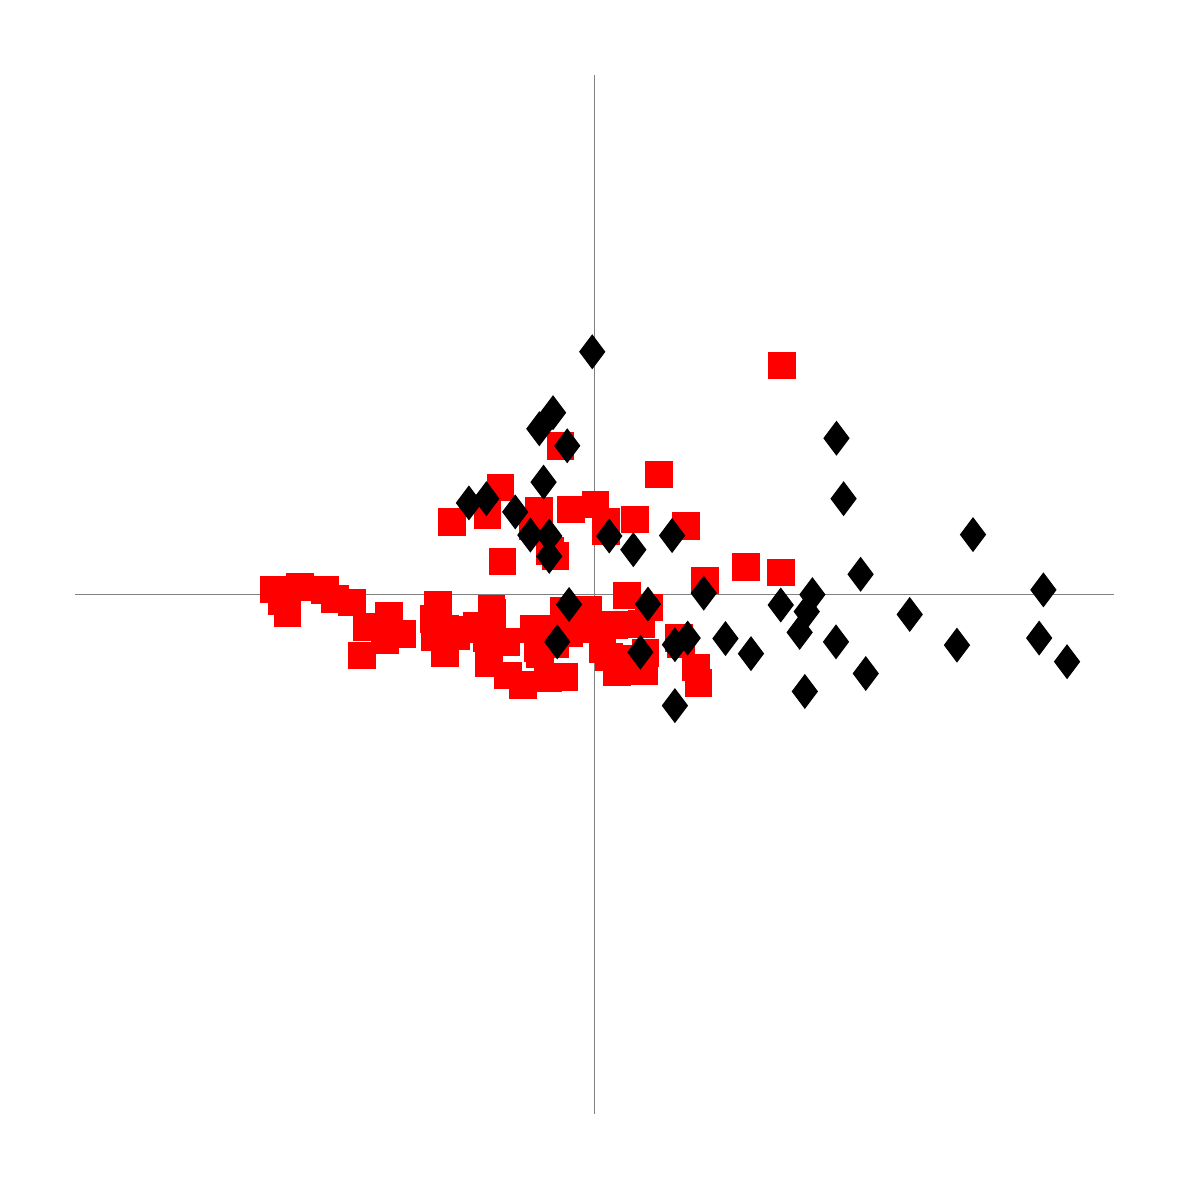
\begin{tikzpicture}[scale=6] \path (-1.2,-1.2) (1.2,1.2);\draw[very thin,color=gray] (0,1.1)--(0,-1.1); \draw[very thin,color=gray] (1.1,0)--(-1.1,0); \path plot[mark=square*,mark options={color=red},mark size=0.8pt] coordinates { (-0.065,-0.035) (-0.331,-0.021) (-0.187,-0.101) (-0.338,-0.090) (-0.129,-0.073) (-0.050,0.180) (0.233,0.030) (-0.492,-0.129) (-0.514,-0.017) (0.012,-0.073) (-0.217,-0.065) (-0.341,-0.051) (0.069,-0.002) (0.396,0.485) (-0.117,0.178) (-0.199,0.227) (-0.115,-0.074) (-0.650,-0.040) (-0.315,-0.078) (0.108,-0.124) (0.215,-0.154) (0.183,-0.104) (0.099,-0.062) (0.321,0.058) (-0.072,-0.072) (0.030,-0.132) (-0.218,-0.031) (-0.084,-0.104) (-0.184,-0.171) (-0.444,-0.096) (-0.317,-0.072) (-0.065,-0.174) (-0.152,-0.192) (0.115,-0.027) (0.086,0.159) (0.136,0.254) (0.002,0.191) (-0.130,0.144) (-0.224,-0.103) (-0.229,-0.093) (0.178,-0.092) (0.042,-0.065) (0.090,-0.147) (0.024,0.155) (0.068,-0.135) (-0.013,-0.033) (0.194,0.145) (0.024,0.134) (0.220,-0.187) (-0.408,-0.084) (-0.317,-0.125) (-0.663,-0.013) (-0.191,-0.100) (-0.115,-0.127) (-0.120,-0.114) (-0.435,-0.044) (0.017,-0.116) (-0.035,-0.069) (-0.054,-0.082) (0.394,0.047) (-0.216,-0.038) (-0.549,-0.009) (-0.678,0.011) (-0.249,-0.067) (-0.292,-0.087) (-0.098,-0.176) (-0.482,-0.068) (0.048,-0.164) (-0.281,-0.074) (-0.570,0.010) (0.105,-0.163) (-0.227,0.168) (-0.094,0.092) (-0.008,-0.073) (-0.195,0.070) (-0.224,-0.146) (-0.623,0.016) (-0.083,0.082) (-0.302,0.154) (-0.072,0.314)};  \path plot[mark=diamond*,mark size=1pt] coordinates { (0.461,-0.000) (0.170,-0.235) (0.563,0.043) (0.801,0.127) (0.950,0.010) (0.767,-0.107) (0.331,-0.125) (0.445,-0.205) (0.511,-0.100) (0.512,0.331) (0.164,0.125) (0.449,-0.036) (0.574,-0.167) (0.667,-0.042) (0.170,-0.106) (-0.108,0.238) (-0.054,-0.021) (0.941,-0.092) (0.277,-0.093) (0.113,-0.020) (0.097,-0.122) (-0.096,0.124) (0.231,0.003) (0.082,0.095) (-0.088,0.385) (0.031,0.124) (-0.168,0.175) (1.000,-0.142) (0.197,-0.092) (0.434,-0.080) (0.394,-0.022) (0.527,0.203) (-0.058,0.315) (-0.266,0.194) (-0.005,0.514) (-0.117,0.351) (-0.096,0.081) (-0.136,0.126) (-0.079,-0.100) (-0.229,0.203)};  \end{tikzpicture} }} & \raisebox{-.5\height}{\resizebox {1.2cm} {1.2cm} { 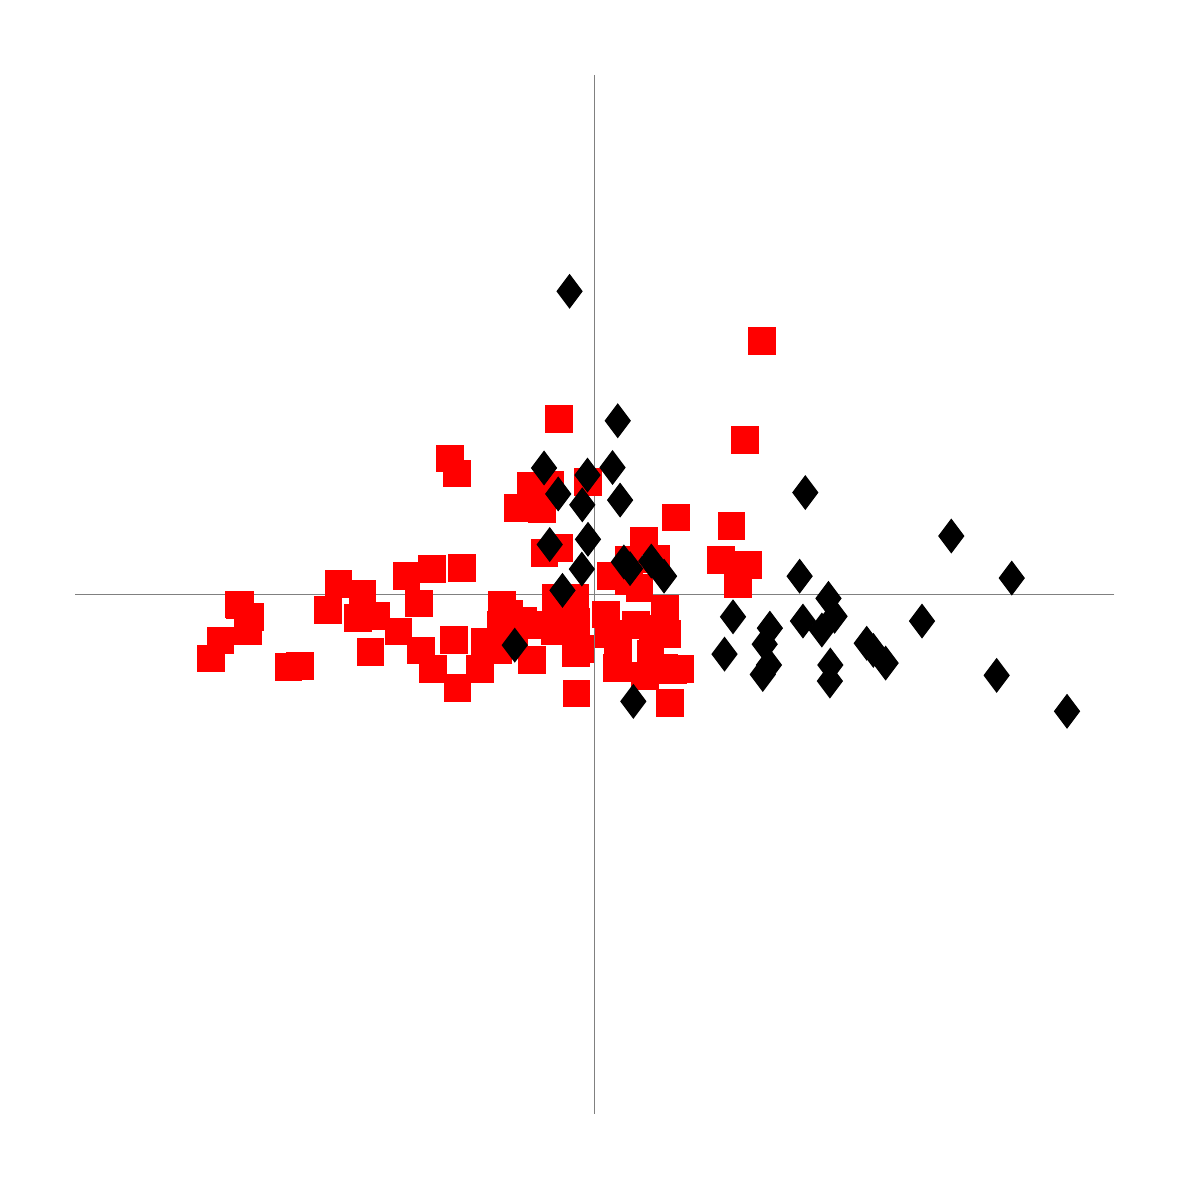
\begin{tikzpicture}[scale=6] \path (-1.2,-1.2) (1.2,1.2);\draw[very thin,color=gray] (0,1.1)--(0,-1.1); \draw[very thin,color=gray] (1.1,0)--(-1.1,0); \path plot[mark=square*,mark options={color=red},mark size=0.8pt] coordinates { (-0.041,-0.007) (-0.542,0.022) (-0.130,-0.065) (-0.564,-0.033) (-0.180,-0.041) (-0.014,0.238) (-0.280,0.057) (-0.623,-0.151) (-0.753,-0.021) (0.087,-0.064) (0.034,0.040) (-0.371,-0.019) (0.072,0.073) (0.355,0.537) (-0.093,0.233) (-0.306,0.288) (0.149,-0.031) (-0.812,-0.135) (-0.297,-0.096) (0.148,-0.155) (0.181,-0.158) (0.153,-0.083) (-0.039,-0.057) (0.303,0.023) (0.123,-0.072) (-0.040,-0.124) (-0.491,0.002) (-0.072,-0.065) (-0.342,-0.158) (-0.474,-0.122) (-0.170,-0.098) (0.107,-0.173) (-0.290,-0.198) (0.095,0.014) (0.173,0.163) (0.318,0.327) (0.290,0.145) (0.131,0.076) (-0.030,-0.114) (-0.082,-0.007) (0.030,-0.083) (0.073,0.029) (0.166,-0.160) (-0.112,0.180) (0.118,-0.126) (-0.196,-0.022) (0.324,0.063) (0.104,0.113) (0.159,-0.229) (-0.196,-0.092) (0.049,-0.119) (-0.734,-0.077) (-0.233,-0.101) (-0.133,-0.138) (-0.205,-0.118) (-0.501,-0.050) (-0.031,-0.115) (-0.199,-0.065) (-0.084,-0.077) (0.267,0.073) (-0.398,0.039) (-0.730,-0.048) (-0.792,-0.097) (-0.463,-0.045) (-0.415,-0.078) (-0.242,-0.157) (-0.648,-0.153) (-0.038,-0.209) (0.024,-0.042) (-0.344,0.054) (0.048,-0.155) (-0.134,0.231) (-0.076,0.098) (-0.151,-0.055) (-0.162,0.183) (-0.367,-0.118) (-0.750,-0.022) (-0.106,0.088) (-0.291,0.256) (-0.075,0.372)};  \path plot[mark=diamond*,mark size=1pt] coordinates { (0.508,-0.046) (0.082,-0.226) (0.434,0.039) (0.883,0.035) (0.693,-0.056) (0.616,-0.145) (0.369,-0.149) (0.356,-0.169) (0.499,-0.149) (0.446,0.216) (0.120,0.071) (0.293,-0.047) (0.498,-0.183) (0.590,-0.118) (0.275,-0.126) (-0.015,0.253) (-0.068,0.009) (0.851,-0.171) (0.371,-0.071) (0.495,-0.008) (0.360,-0.105) (-0.095,0.106) (0.075,0.055) (0.062,0.069) (0.049,0.368) (0.147,0.039) (-0.077,0.213) (1.000,-0.247) (0.576,-0.103) (0.481,-0.075) (0.441,-0.056) (0.755,0.124) (0.038,0.269) (0.054,0.200) (-0.053,0.642) (-0.107,0.268) (-0.027,0.054) (-0.014,0.117) (-0.169,-0.107) (-0.026,0.190)};  \end{tikzpicture} }} & \raisebox{-.5\height}{\resizebox {1.2cm} {1.2cm} { 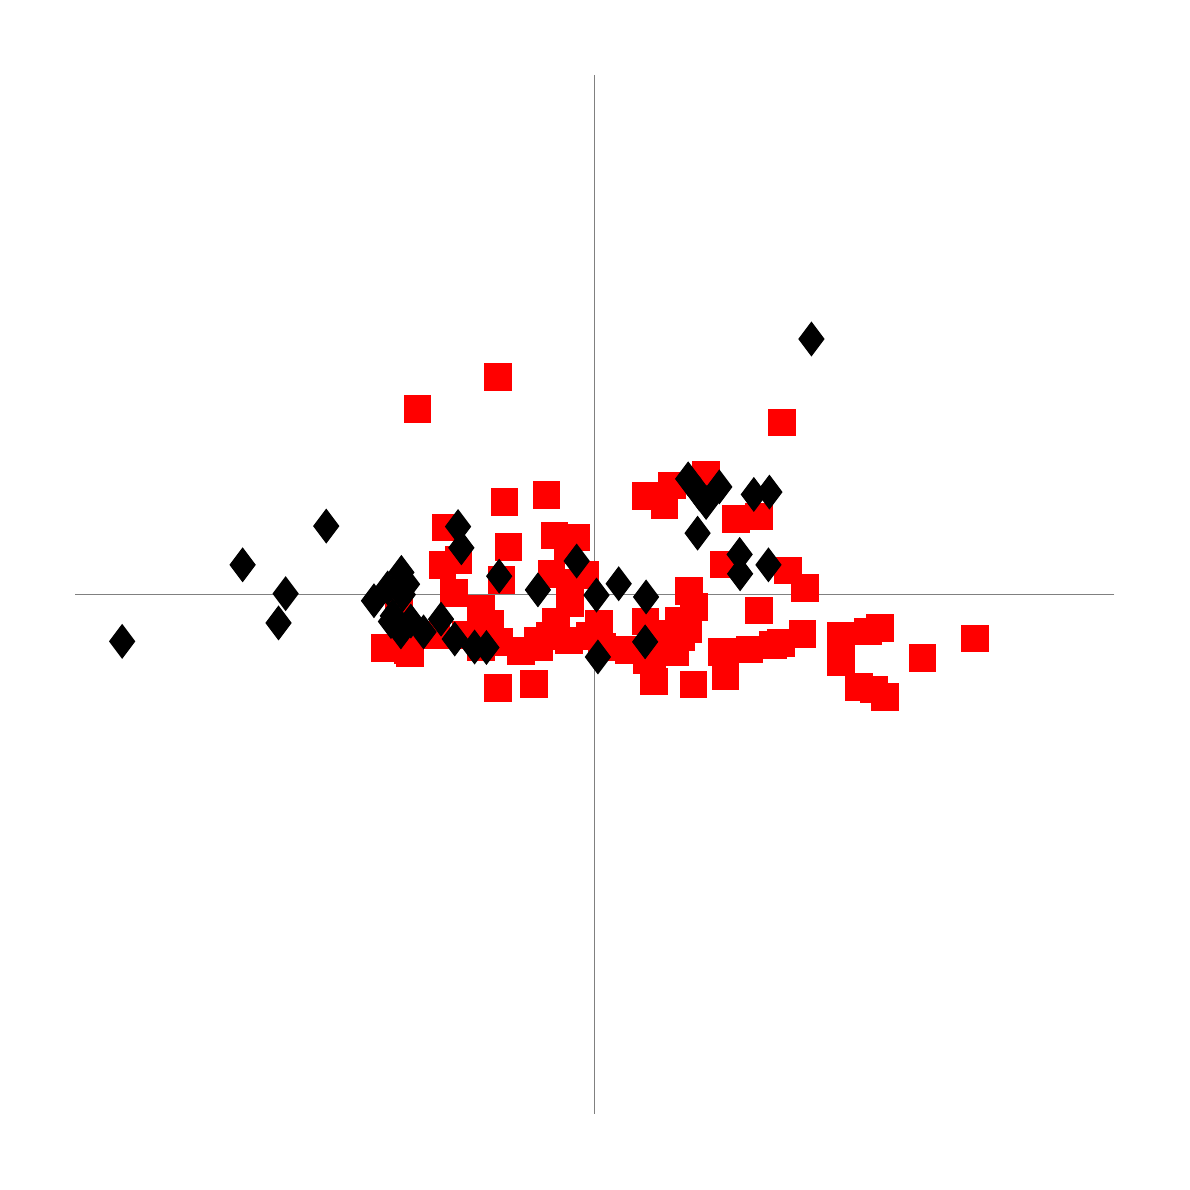
\begin{tikzpicture}[scale=6] \path (-1.2,-1.2) (1.2,1.2);\draw[very thin,color=gray] (0,1.1)--(0,-1.1); \draw[very thin,color=gray] (1.1,0)--(-1.1,0); \path plot[mark=square*,mark options={color=red},mark size=0.8pt] coordinates { (-0.052,-0.019) (0.604,-0.070) (0.108,-0.057) (0.579,-0.078) (0.211,-0.026) (-0.102,0.211) (0.348,-0.034) (0.560,-0.195) (0.805,-0.093) (-0.082,-0.058) (-0.182,0.101) (0.197,-0.074) (-0.057,0.094) (-0.204,0.461) (0.109,0.209) (0.348,0.165) (-0.298,0.004) (0.592,-0.201) (0.120,-0.111) (-0.156,-0.120) (-0.240,-0.111) (-0.222,-0.062) (0.191,-0.059) (-0.091,0.043) (-0.241,-0.031) (-0.117,-0.112) (0.522,-0.087) (0.009,-0.062) (0.277,-0.172) (0.209,-0.190) (-0.203,-0.101) (-0.444,-0.113) (0.126,-0.184) (-0.020,0.042) (-0.191,0.196) (-0.375,0.393) (-0.315,0.142) (-0.197,0.031) (-0.273,-0.085) (-0.052,0.024) (-0.054,-0.097) (-0.322,0.063) (-0.391,-0.124) (0.299,0.160) (-0.121,-0.097) (0.179,-0.056) (-0.288,0.073) (-0.040,0.121) (-0.205,-0.198) (-0.095,-0.087) (-0.336,-0.085) (0.269,-0.121) (0.140,-0.101) (0.015,-0.111) (0.171,-0.122) (0.394,-0.103) (0.072,-0.117) (0.184,-0.090) (-0.010,-0.088) (-0.085,0.125) (0.445,0.014) (0.694,-0.134) (0.522,-0.142) (0.440,-0.083) (0.328,-0.116) (0.121,-0.139) (0.615,-0.217) (-0.128,-0.189) (-0.414,-0.015) (0.200,0.007) (-0.396,-0.117) (0.236,0.254) (0.274,0.064) (0.122,-0.084) (0.148,0.190) (0.111,-0.139) (0.377,-0.107) (0.410,0.051) (0.164,0.231) (0.397,0.364)};  \path plot[mark=diamond*,mark size=1pt] coordinates { (-0.427,-0.045) (0.007,-0.132) (-0.282,0.099) (-0.745,0.063) (-0.409,0.047) (-0.467,-0.013) (-0.254,-0.111) (-0.229,-0.112) (-0.362,-0.079) (-0.289,0.144) (-0.202,0.039) (0.004,-0.001) (-0.389,-0.056) (-0.431,-0.057) (-0.296,-0.094) (0.222,0.213) (0.051,0.023) (-0.669,-0.060) (-0.438,0.014) (-0.397,0.022) (-0.410,-0.079) (0.368,0.063) (-0.038,0.071) (-0.120,0.010) (0.198,0.245) (0.109,-0.005) (0.264,0.228) (-1.000,-0.099) (-0.654,0.002) (-0.406,0.000) (-0.325,-0.052) (-0.568,0.145) (0.337,0.212) (0.236,0.195) (0.459,0.541) (0.307,0.085) (0.308,0.044) (0.218,0.130) (0.107,-0.100) (0.370,0.217)};  \end{tikzpicture} }} & \raisebox{-.5\height}{\resizebox {1.2cm} {1.2cm} { 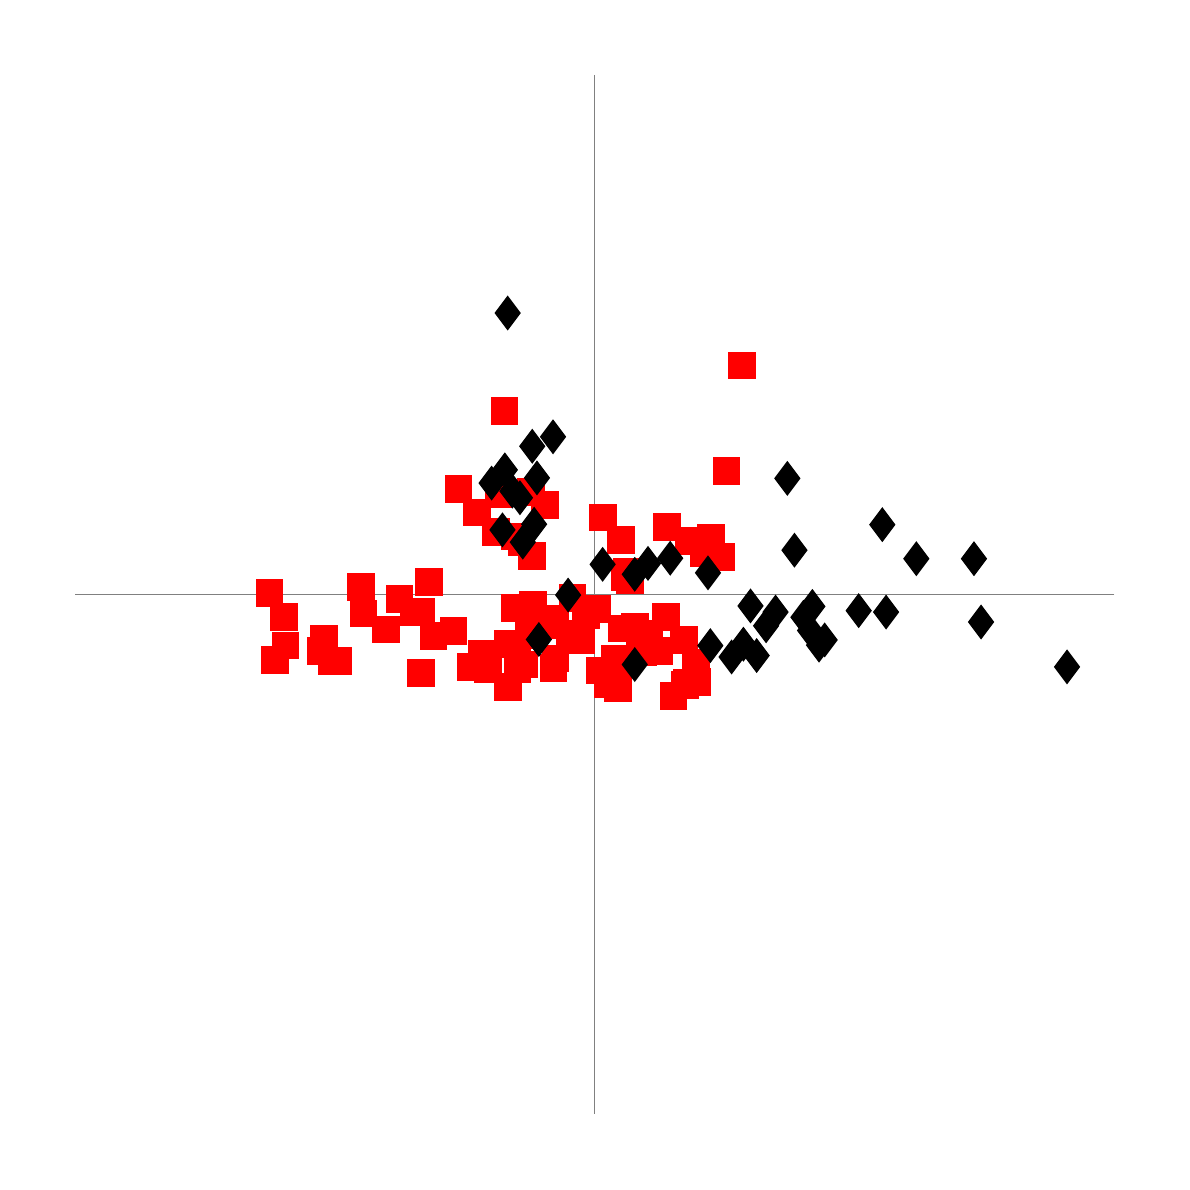
\begin{tikzpicture}[scale=6] \path (-1.2,-1.2) (1.2,1.2);\draw[very thin,color=gray] (0,1.1)--(0,-1.1); \draw[very thin,color=gray] (1.1,0)--(-1.1,0); \path plot[mark=square*,mark options={color=red},mark size=0.8pt] coordinates { (-0.018,-0.043) (-0.495,0.016) (-0.139,-0.086) (-0.489,-0.040) (-0.169,-0.029) (0.018,0.163) (-0.133,0.081) (-0.556,-0.141) (-0.688,0.003) (0.058,-0.072) (0.005,-0.031) (-0.299,-0.077) (0.068,0.049) (0.312,0.485) (-0.105,0.190) (-0.288,0.224) (0.115,-0.082) (-0.676,-0.138) (-0.239,-0.125) (0.137,-0.120) (0.215,-0.144) (0.189,-0.096) (-0.047,-0.007) (0.231,0.087) (0.096,-0.082) (0.042,-0.137) (-0.413,-0.009) (-0.053,-0.084) (-0.262,-0.153) (-0.367,-0.166) (-0.087,-0.156) (0.167,-0.215) (-0.183,-0.195) (0.075,0.030) (0.153,0.143) (0.279,0.262) (0.200,0.113) (0.064,0.037) (0.012,-0.161) (-0.084,-0.064) (0.086,-0.068) (0.151,-0.047) (0.218,-0.185) (-0.134,0.217) (0.103,-0.122) (-0.130,-0.021) (0.268,0.079) (0.056,0.115) (0.195,-0.186) (-0.163,-0.157) (0.027,-0.190) (-0.543,-0.141) (-0.184,-0.105) (-0.083,-0.135) (-0.163,-0.108) (-0.441,-0.074) (-0.028,-0.096) (-0.138,-0.057) (-0.039,-0.087) (0.246,0.121) (-0.350,0.026) (-0.657,-0.047) (-0.654,-0.108) (-0.383,-0.038) (-0.341,-0.088) (-0.149,-0.148) (-0.580,-0.119) (0.050,-0.198) (0.058,-0.139) (-0.368,-0.037) (0.191,-0.192) (-0.202,0.212) (-0.155,0.112) (-0.091,-0.052) (-0.168,0.123) (-0.226,-0.157) (-0.573,-0.094) (-0.208,0.133) (-0.249,0.174) (-0.191,0.389)};  \path plot[mark=diamond*,mark size=1pt] coordinates { (0.461,-0.025) (0.085,-0.148) (0.423,0.094) (0.803,0.076) (0.681,0.076) (0.617,-0.037) (0.315,-0.105) (0.343,-0.129) (0.456,-0.076) (0.408,0.246) (0.160,0.077) (0.240,0.046) (0.487,-0.096) (0.559,-0.034) (0.245,-0.108) (-0.122,0.247) (-0.056,-0.001) (0.818,-0.058) (0.363,-0.066) (0.330,-0.024) (0.290,-0.132) (-0.195,0.137) (0.113,0.066) (0.085,0.043) (-0.088,0.334) (0.017,0.064) (-0.174,0.219) (1.000,-0.153) (0.475,-0.107) (0.442,-0.048) (0.383,-0.037) (0.609,0.148) (-0.132,0.314) (-0.158,0.205) (-0.184,0.596) (-0.190,0.264) (-0.152,0.111) (-0.128,0.149) (-0.118,-0.095) (-0.218,0.236)};  \end{tikzpicture} }}\\
\bottomrule
\end{tabular}



\end{table}

\end{document}
